
This module deals with the delivery of information regarding the device and its cats to the owner (user) of the device via the Internet. Following are the required features:

\begin{itemize}
    \item Device's food supply level
    \item Device's battery level during charging
    \item Device's battery level during operation
    \item Device's feeding log
    \item Cats' profiles
\end{itemize}

An explanation and reasoning of the requirements is due:

\textbf{Food Supply: } Food supply level information helps the user decide when to refill the food tank. How the information is obtained is explained in detail in Section \ref{sec:electrical_design}.

\textbf{Battery Level: } This is essential for any rechargeable product. Detailed explanation will follow in Section \ref{sec:electrical_design}.

\textbf{Feeding log: } Each device has a feeding log of all cats that have been fed from it since its setup.

\textbf{Cat profiles: } These profiles are initially handled by the Identification module. (see 4.\ref{sec:identification}. Each profile includes a name, an image and an individual feeding log. Furthermore, the name attribute is initially 'name' and can be edited later on by the user of the device. Nonetheless, the user cannot edit his/her cats' images: the images are provided by the device's camera. Feeding log is also not to be edited.

% justify istiyor iste, biliyordum falan diyebilirsin tecrubem vardi, cpu time dusuk falan, ek sunucu ihtiyaci yok, python ile iletisim kuruyor

For the interface, a Python web framework called Flask is used. There were a few reasons behind this choice:

\begin{itemize}
    \item Our user interface and web designer, Furkan, had more experience in Flask than in other frameworks.
    \item Since Flask uses Python in the background, CPU time is less than other platforms such as Nodejs.
    \item There is no need for an additional server, since a command as simple as `flask run' can let us run our website on our computers.
    \item Because the communicated modules are mostly developed in Python, the communication is seamless.
\end{itemize}

The user interface, prototype of which is currently hosted on \\ \href{https://felerest.pythonanywhere.com/}{felerest.pythonanywhere.com}, consists of 3 main pages: devices page, cats page, settings page, all of which can be accessed only with the user's password.

\clearpage

\begin{figure}[ht] 
     \centering
     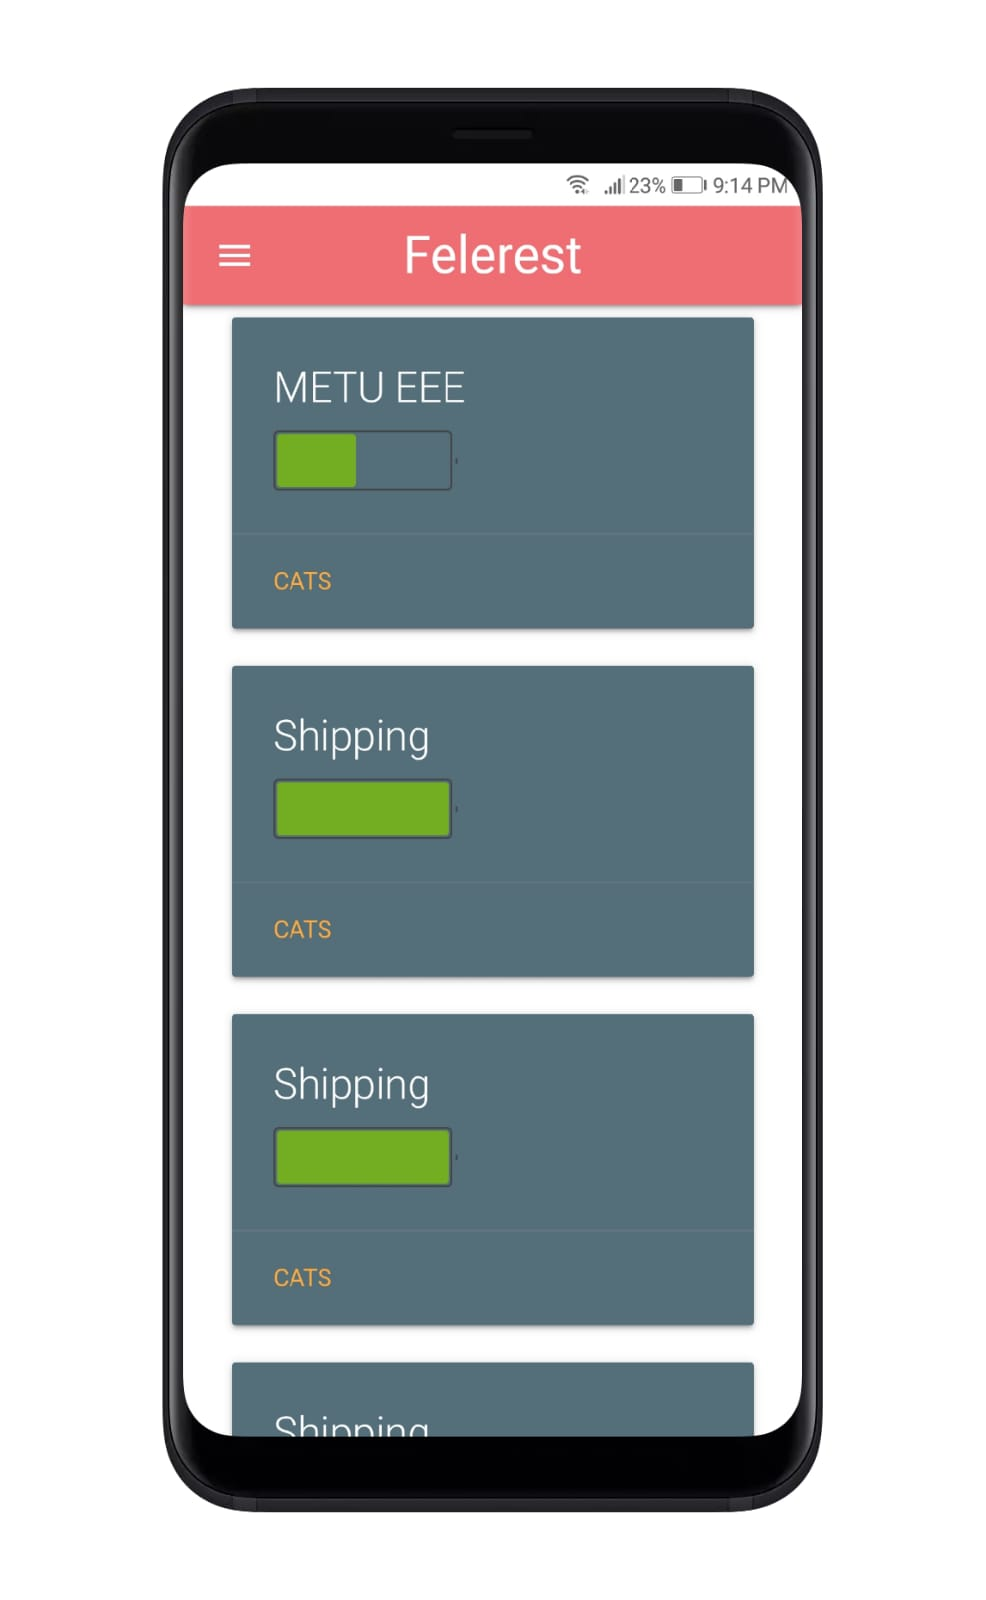
\includegraphics[width=.55\linewidth]{content/030_system_architecture/img/user_interface/devices.jpeg}
     \caption{User Devices Page}
     \label{fig:ui-devices}
\end{figure}

The devices page (Figure \ref{fig:ui-devices}) displays all devices that the user owns as cards in a grid. Each card shows that particular device's location, battery level, and food supply level. The food supply level indicator will be added eventually. There is also a link at the bottom of each card that takes the user to that device's cats page. There will also be another link that displays the entire feeding log of the device.

Cards in the figure labeled Shipping are just dummy devices to test the behavior of the grid with multiple cards.


\begin{figure}[ht]

\begin{subfigure}{0.5\textwidth}
    \centering
    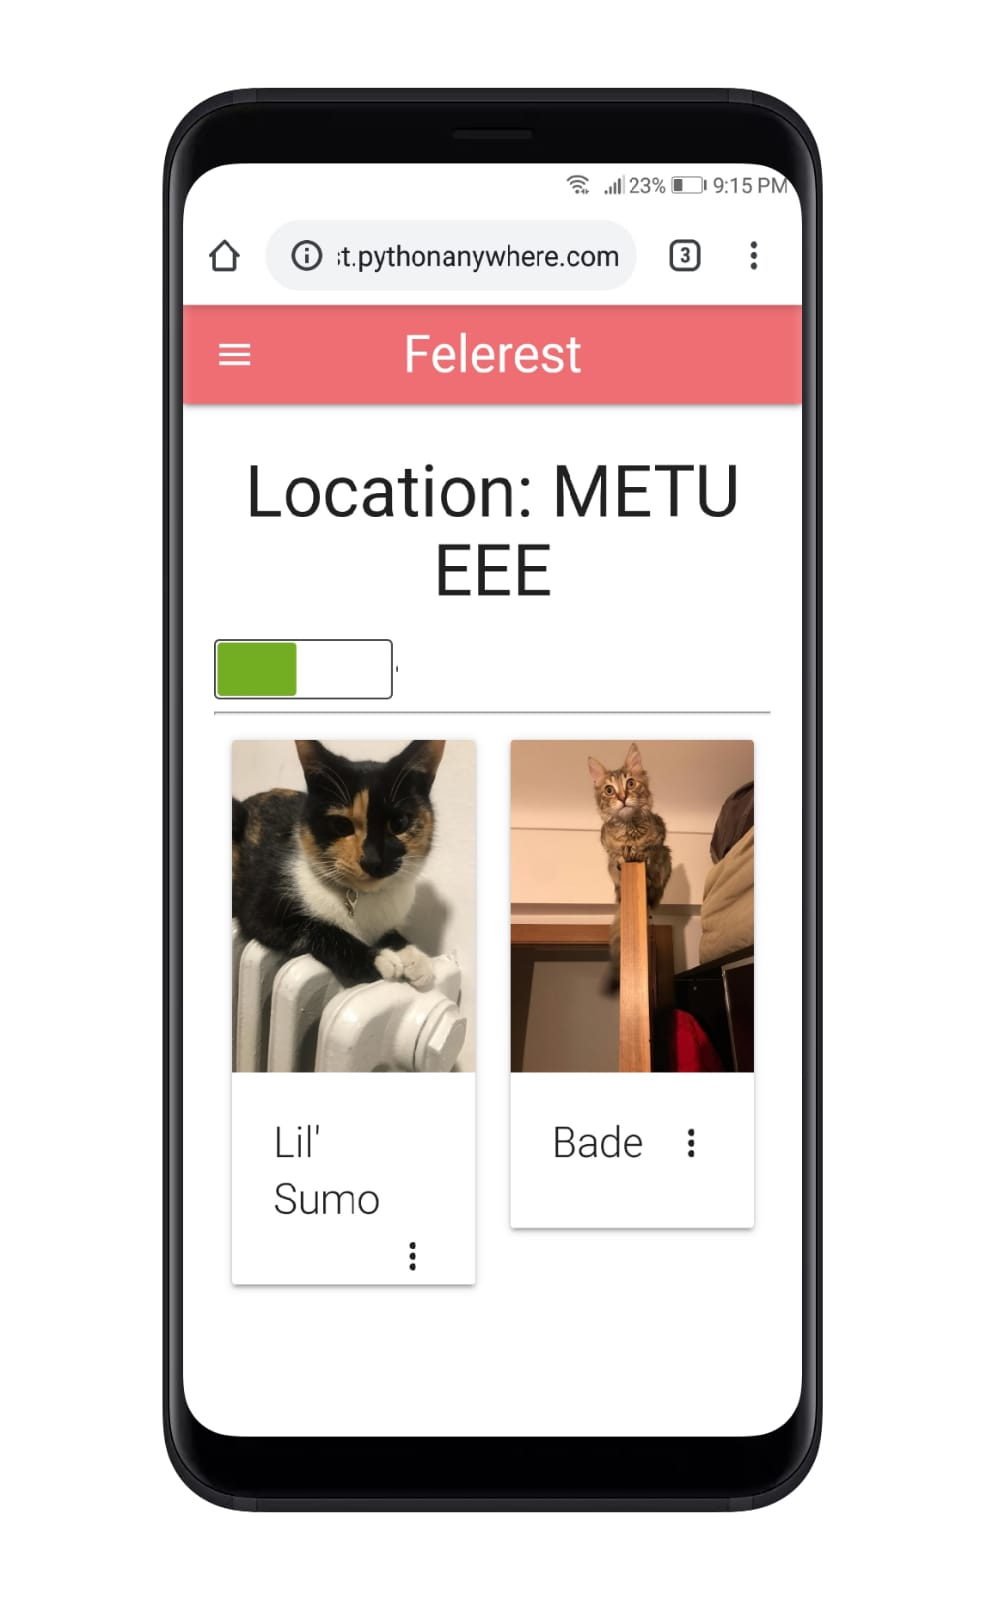
\includegraphics[width=\linewidth]{content/030_system_architecture/img/user_interface/cats.jpeg}
    \caption{Device Cats Non-revealed}
    \label{fig:ui-cats}
\end{subfigure}
\begin{subfigure}{0.5\textwidth}
    \centering
    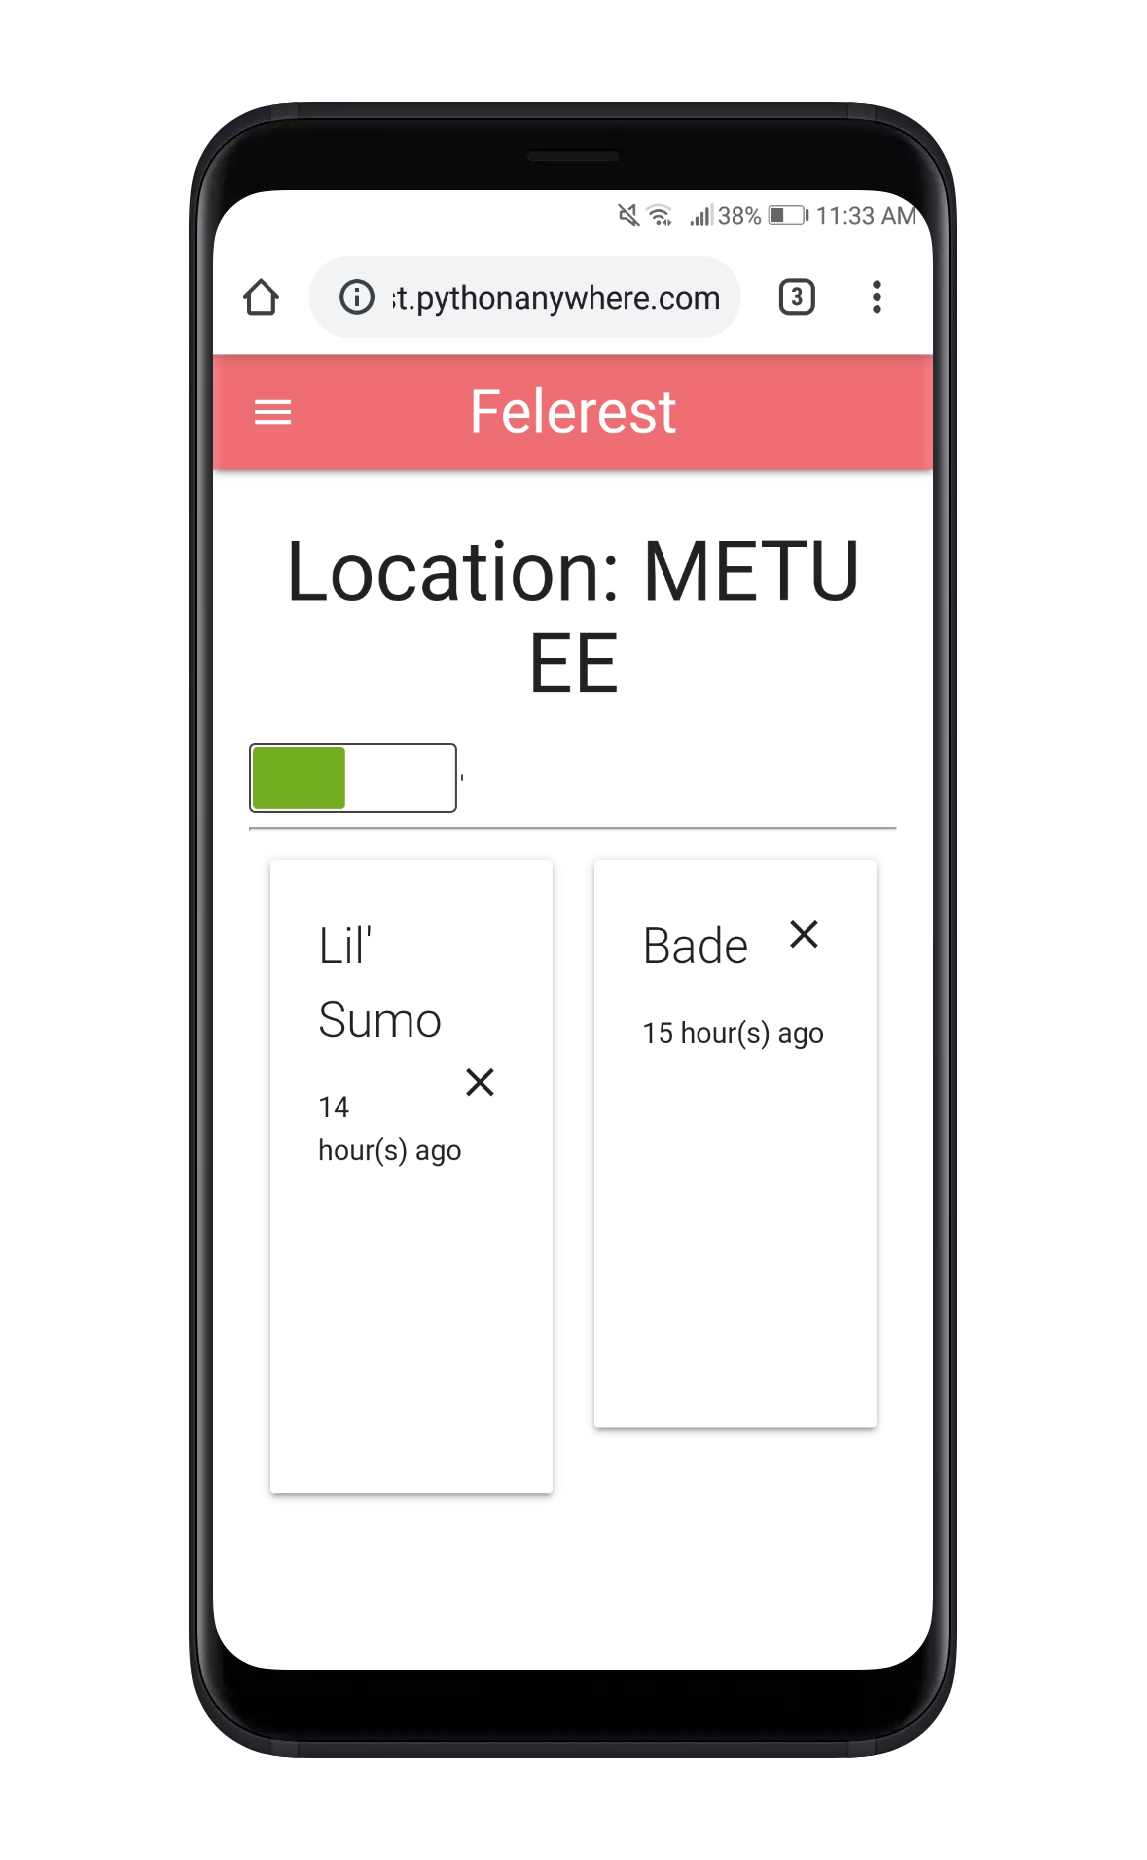
\includegraphics[width=\linewidth]{content/030_system_architecture/img/user_interface/cats_revealed.png}
    \caption{Device Cats Revealed}
    \label{fig:ui-cats-revealed}
\end{subfigure}
\caption{Device Cats Page}
    \label{fig:ui-cats-combined}
\end{figure}

The cats page (Figure \ref{fig:ui-cats-combined}) displays all cats that belongs to a device. On the page, the location, battery level, and food supply level of the device is displayed again for convenience of the user. Moreover, each cat has its own card that displays a name and an image. When the user clicks on a cat's card, the last feeding time of the cat is revealed, along with a link to the cat's feeding log. Currently, only the last feeding time is implemented.

\begin{figure}[h!] 
     \centering
     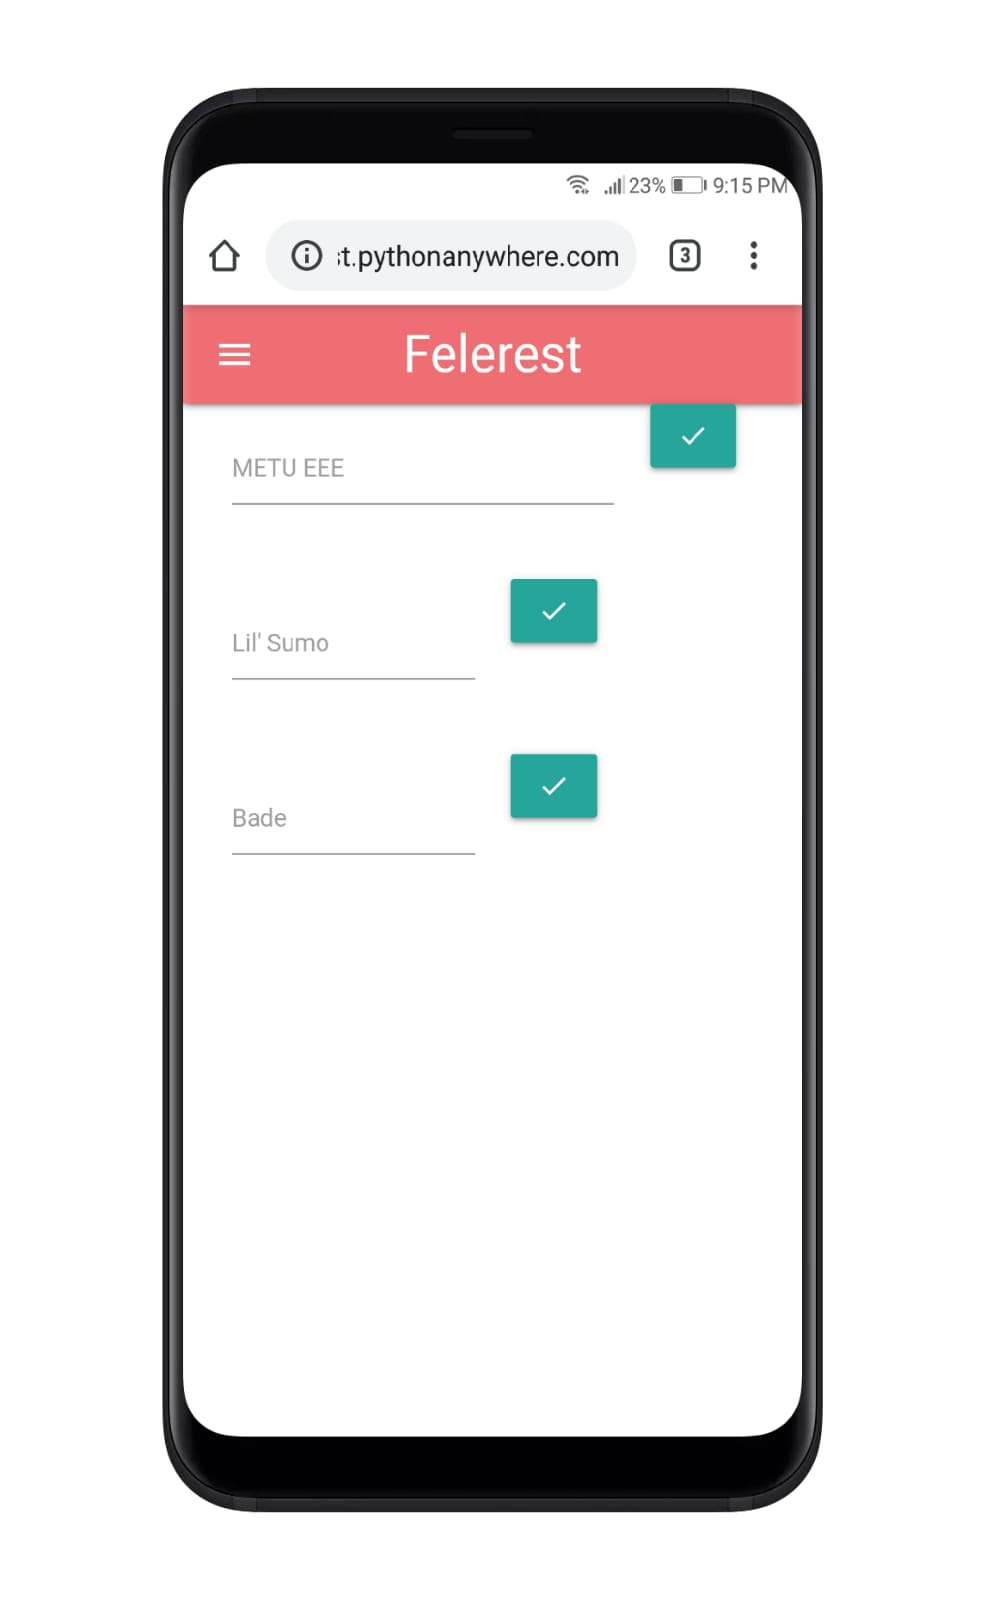
\includegraphics[width=.55\linewidth]{content/030_system_architecture/img/user_interface/settings.jpeg}
     \caption{User Account (Settings) Page}
     \label{fig:ui-settings}
\end{figure}

The last essential page, the settings page, can be seen in Figure \ref{fig:ui-settings}. Here the user can change the locations of devices and names of cats that are affiliated with him/her. The changes that are done here are implemented instantly. Locations/names `METU EEE', `Lil' Sumo', and `Bade' have all been given as inputs to this page.

\clearpage
